\section{Camera calibration} 10 RBG images were fed into the OpenCV algorithm for camera calibration. Calibration results along with the factory setting values are given in the below table.

\begin{table}[hbt]
	\centering
	\begin{tabular}{|c|c|c|}
		\hline
		Parameters & calibrated values & Factory calibration settings\\ 
		\hline
		$\alpha_x$  & \num{968.7}  & \num{971.99}\\
		$\alpha_y$ & \num{968.9} & \num{971.906}\\
		S & 0.0 & 0.0\\
		$C_x$ & \num{1026} & \num{1022.58} \\
		$C_y$ & \num{774.0} & \num{775.268} \\
		$K_1$ & \num{0.07588} & \num{0.781141} \\
		$K_2$ & \num{0.04285}  & \num{-3.0437}\\
		$P_1$ & \num{-0.00064} & \num{0.000616}\\
		$P_2$ & \num{0.00132}  & \num{-2.35e-05} \\
		$K_3$ & \num{-0.25794} & \num{1.7224} \\
		\hline
	\end{tabular}
	\caption{Microsoft azure kinect calibration result}
	\label{tab:kinect_camera_calibration_result}
\end{table}

\section{Hand-eye calibration}

We have achieved a high degree of accuracy in estimating 2 unknowns in the hand-eye calibration equation i.e camera position and marker position. Both Microsoft Kinect and Atracsys fusionTrac 500 hand-eye calibration resulted in positional error < 1.5 millimeters and rotational error < 0.3 degrees on a hold-out validation set as shown in the \cref{tab:kinect__fusionTrac_handeye_result}.

\begin{table}[hbt!]
	\centering
	\begin{tabular}{|c|c|c|}
		\hline
		Camera & Translation error (m) & Rotational error ($\deg$)\\ 
		\hline
		Kinect & 0.001$\pm$ $\num{1.40e-07}$  & 0.258 $\pm$ $\num{0.0}$\\
		fusionTrac & 0.001 $\pm$ $\num{2.8e-07}$  & 0.205 $\pm$ $\num{0.0}$\\
		\hline
	\end{tabular}
	\caption{Hand-eye calibration results}
	\label{tab:kinect__fusionTrac_handeye_result}
\end{table}

\section{Head coordinate system} Head coordinate system is created with the 3 anatomoical feature of the face (RPA, nose $ \& $ LPA ) We can map above points to coordinate system to check whether we have right coordinate system. By observing the translational part expressed in head coordinate system  $\tfMat{H_{cs}}{T}{RPA}$, $\tfMat{H_{cs}}{T}{nasion}$ $\&$ $\tfMat{H_{cs}}{T}{LPA}$ respectively it is indeed that and RPA, nasion, LPA make the 3 perpendicular axis. The \cref{fig:head_coordinate} shows these points graphically, RPA is at 56.5mm along -$\vect{y}$ axis, nasion is at 97.6mm along $\vect{x}$ axis, and LPA is at 74.6mm along $\vect{y}$ axis. 

\begin{equation*} 
	\centering
	\begin{bmatrix}
		0.0 \\
		-0.0565\\
		\num{2.775e-17}\\
	\end{bmatrix}
\end{equation*}

\begin{equation*} 
	\centering
	\begin{bmatrix}
		0.0976\\
		\num{2.775e-17}\\
		0.0\\
	\end{bmatrix}
\end{equation*}

\begin{equation*} 
	\centering
	\begin{bmatrix}
		0.0\\
		0.0746\\
	    0.0\\
	\end{bmatrix}
\end{equation*}

\begin{figure}[hbt!]
	\centering
	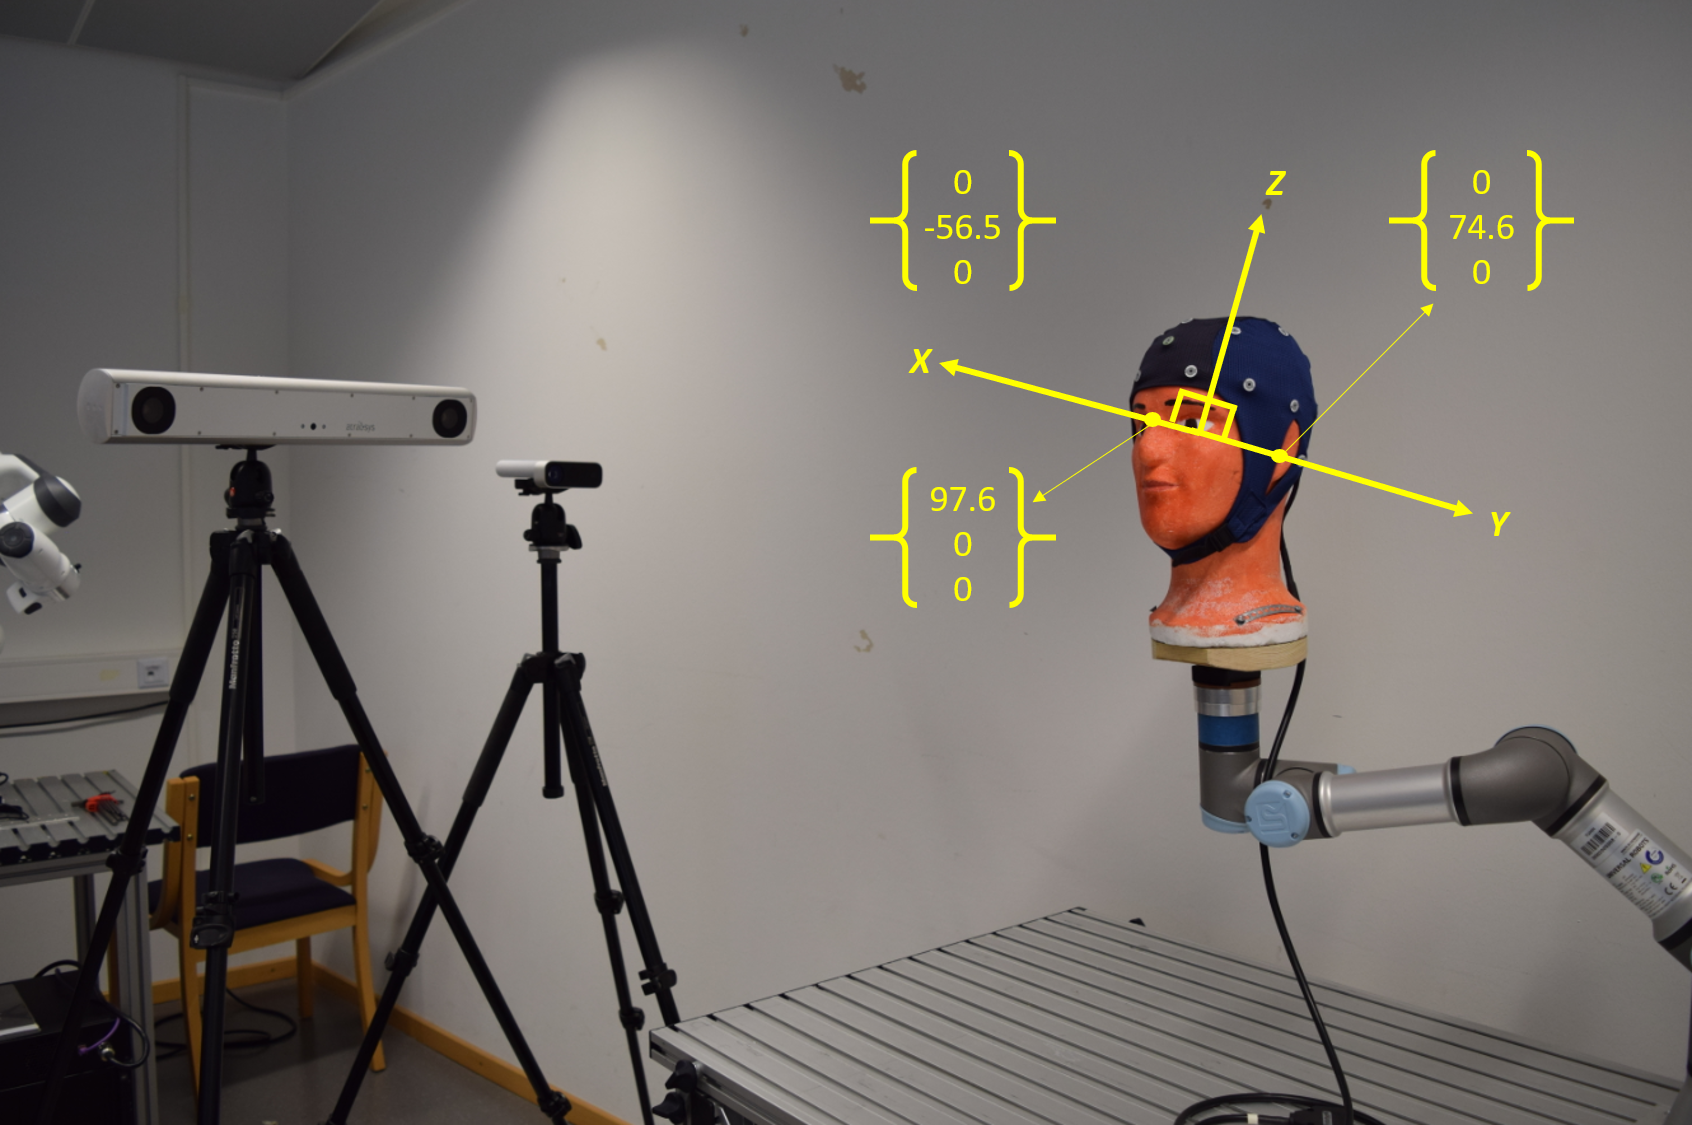
\includegraphics[width=\linewidth]{head_coordinate.png}
	\caption{Head coordinate system using RPA, nose and LPA} 
	\label{fig:head_coordinate}
\end{figure}

\section{Accuracy of the data acquisition system}

\begin{figure}[hbt!]
	\centering
	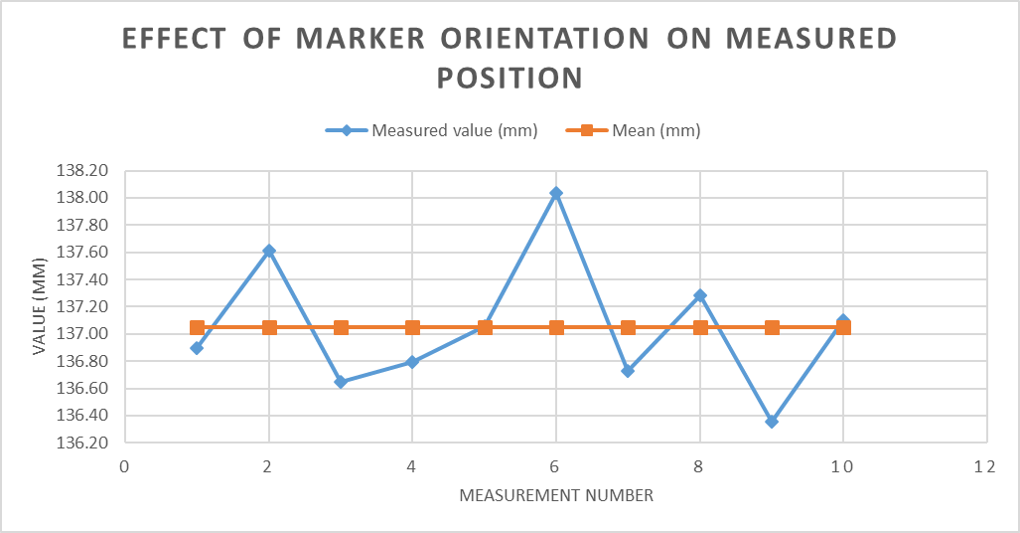
\includegraphics[scale=0.8]{active_marker_positional_error_normalised.png}
	\caption{Measurement of single electrode with ten different marker orientation} 
	\label{fig:active_marker_normalised_positional_error}
\end{figure}

The \cref{fig:active_marker_normalised_positional_error} shows the ten measurements of the same electrode with different marker orientation with mean value 137.05 $\pm$ 1 mm, therefore, we conclude that the measurement error due to the orientation of the marker is negligible.  

\begin{figure}[hbt!]
	\centering
	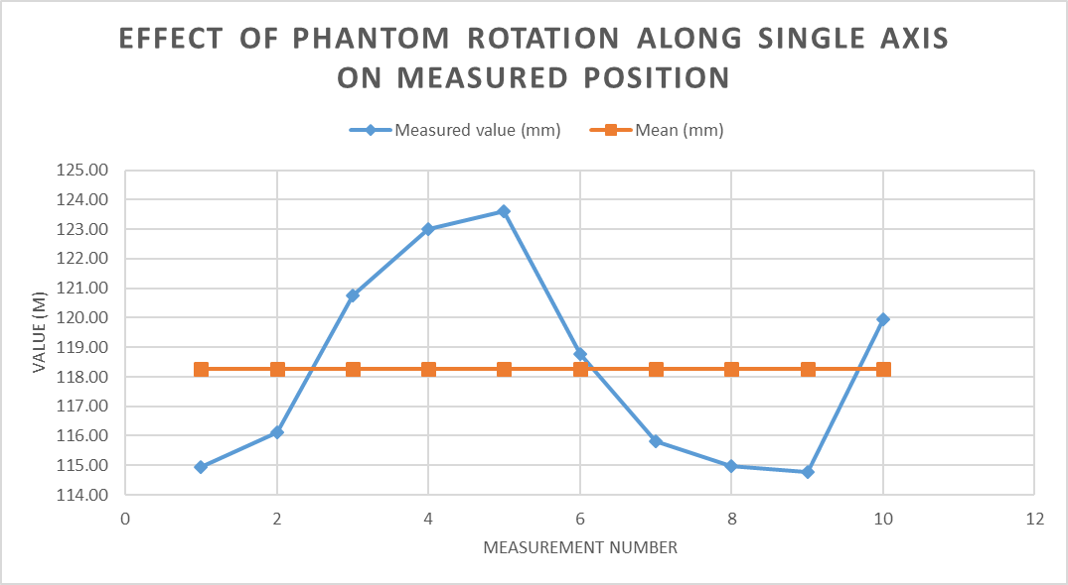
\includegraphics[scale=0.8]{normalised_positional_error_single_axis.png}
	\caption{Measurement of single electrode when phantom head roatated to ten different angles along an axis.} 
	\label{fig:Normalised_positional_error_single_axis}
\end{figure}

The \cref{fig:Normalised_positional_error_single_axis} shows the ten measurements for single axis phantom rotation with mean value 118.26$\pm$4.5mm. 

\begin{figure}[hbt!]
	\centering
	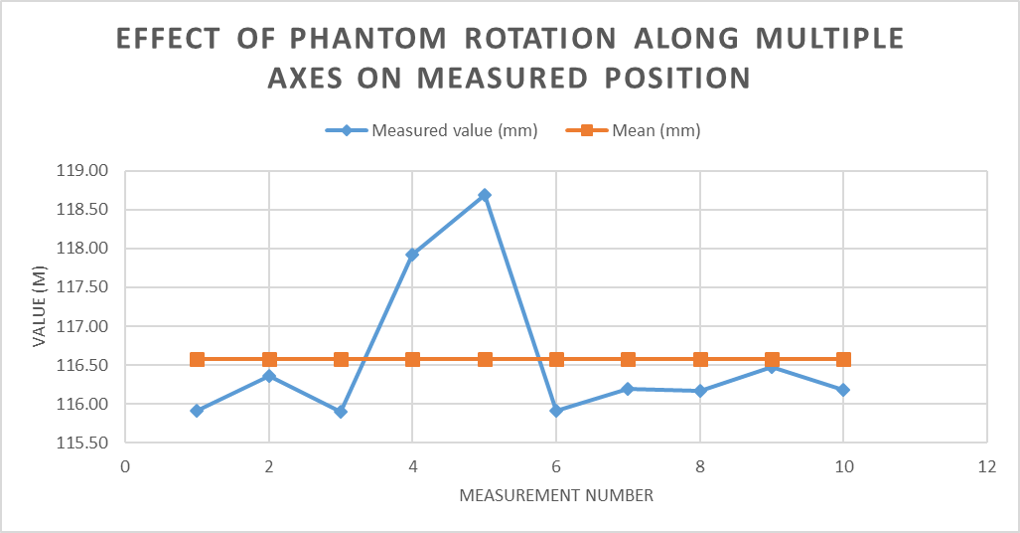
\includegraphics[scale=0.8]{normalised_positional_error_multiple_axis.png}
	\caption{Measurement of single electrode when phantom head roatated to ten different angles along multiple axes.}  
	\label{fig:Normalised_positional_error_multiple_axis}
\end{figure}

The \cref{fig:Normalised_positional_error_multiple_axis} shows the ten measurements for multiple axis phantom movement with 116.5$\pm$ 1.5mm therefore, we conclude this robotic system can generate ground truth data with accuracy of $\approx$ $\pm$ 5mm.

\hfill
\newpage
\section{Range of electrode position variation}
To evaluate the extent to which electrodes position varies at different wearing instances of the EEG cap, we tried to simulate attaching the EEG cap on the phantom for 5 times and measure the variance of the electrode position. \cref{fig:blue_cap_all} and \cref{fig:blue_cap_all_side_view} shows the electrode position at 5 such instances.
\begin{figure}[hbt!]
	\centering
	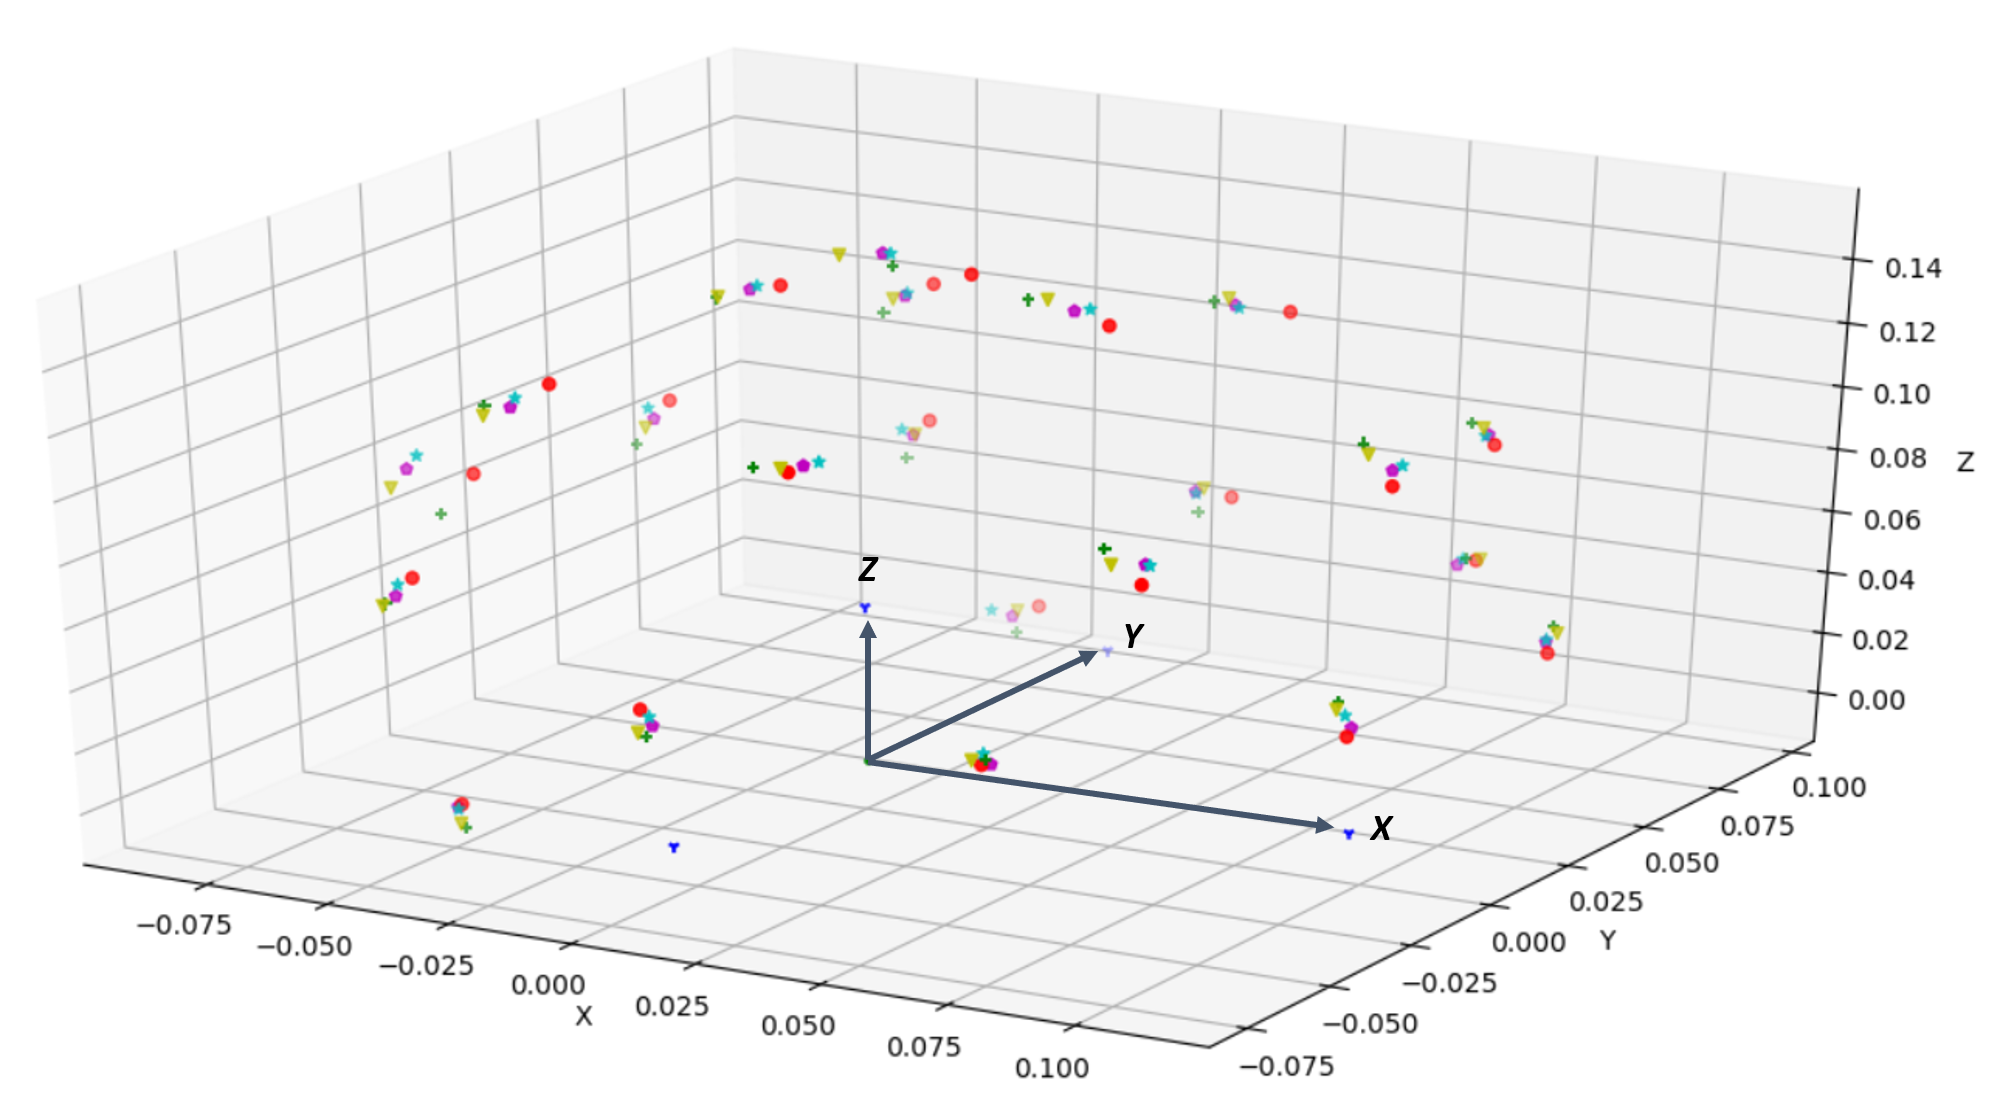
\includegraphics[width=\linewidth]{blue_cap_all.png}
	\caption{3D view of electrodes at 5 different EEG cap wearing instances} 
	\label{fig:blue_cap_all}
\end{figure}

\begin{figure}[hbt!]
	\centering
	\begin{subfigure}{0.49\textwidth}
		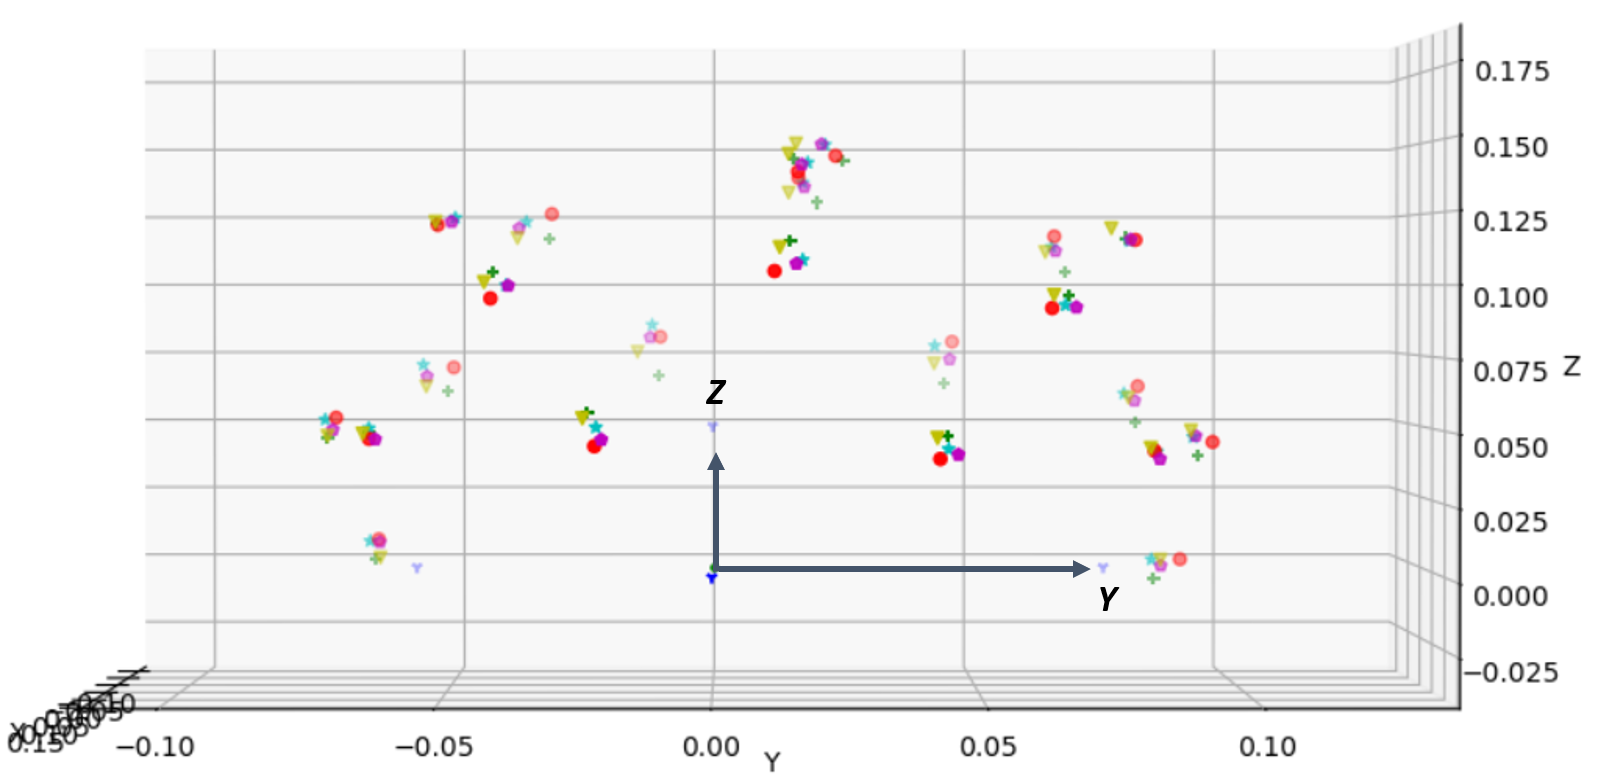
\includegraphics[width=\textwidth]{blue_cap_all_side_view_1.png}	
	\end{subfigure}
	\hfill
	\begin{subfigure}{0.49\textwidth}
		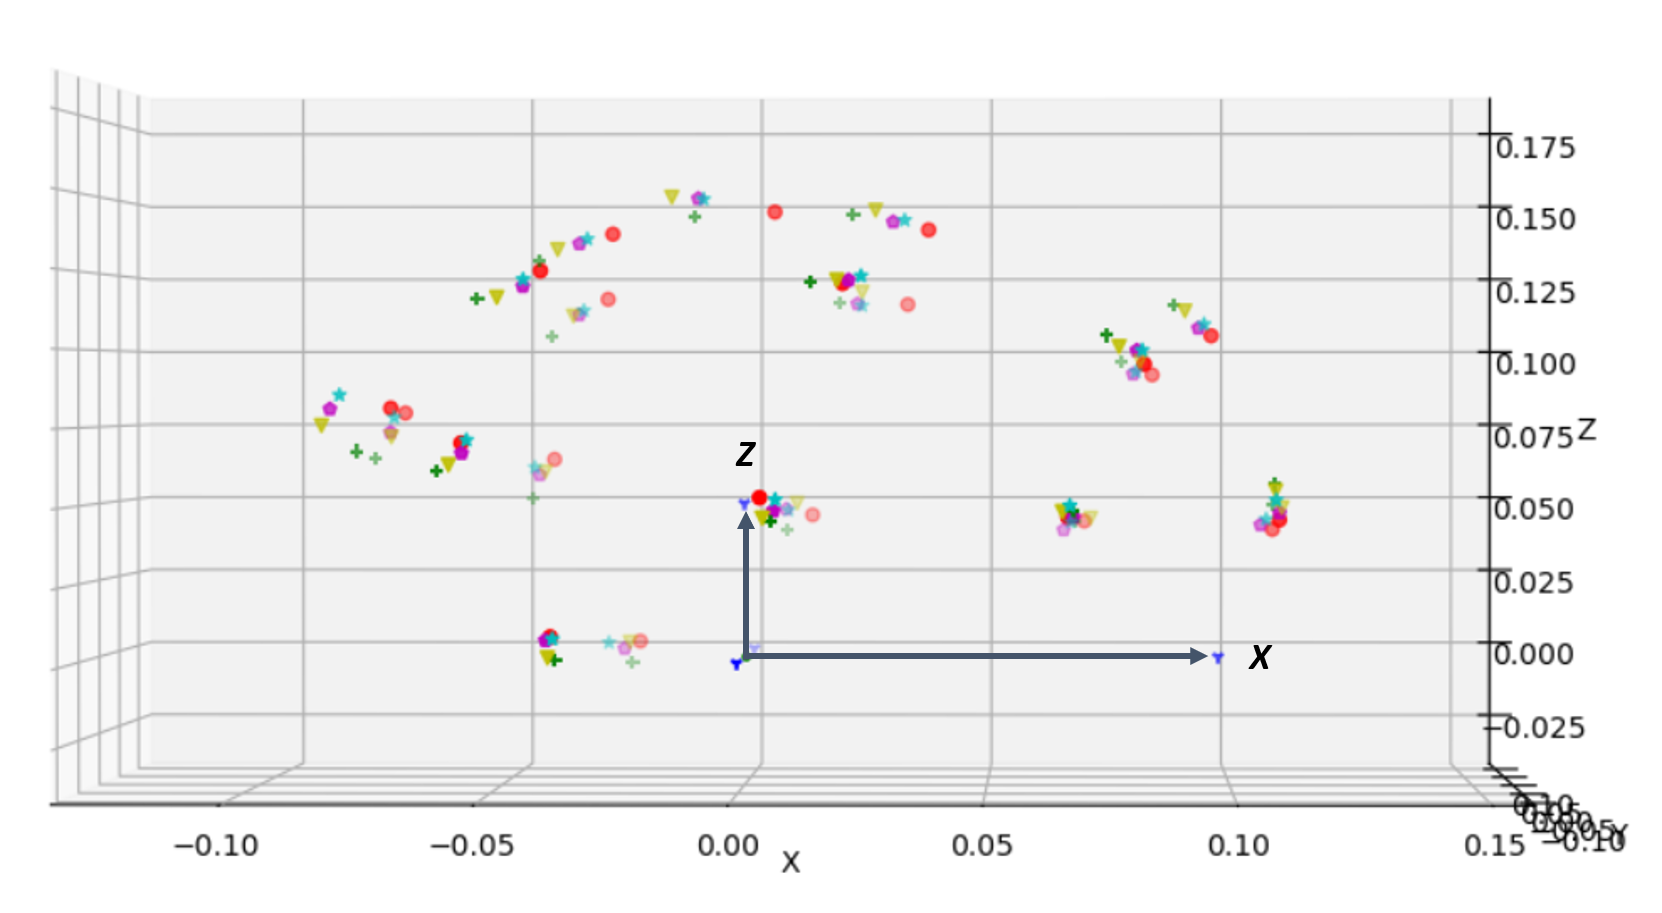
\includegraphics[width=\textwidth]{blue_cap_all_side_view_2.png}	
	\end{subfigure}
	\caption{2D side views of electrodes at 5 different EEG cap wearing instances} 
	\label{fig:blue_cap_all_side_view}
\end{figure} 

\hfill
\newpage
The \cref{fig:electrode_position_range} shows the range of electrode position variation during 5 electrode wearing instances to be with mean value 7.8 $\pm$ 5.8 mm.
\begin{figure}[ht!]
	\centering
	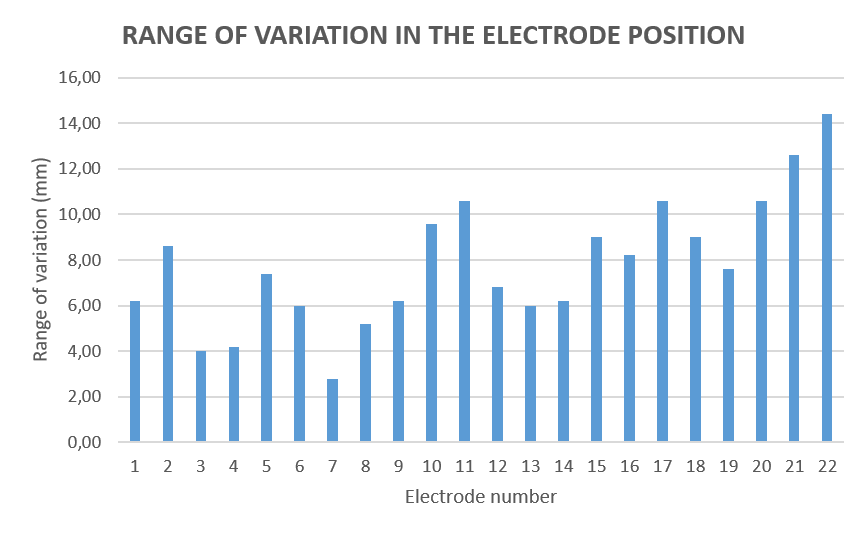
\includegraphics[scale=0.8]{electrode_position_range.png}
	\caption{Range of electrode position variation at 5 different EEG cap wearing instances} 
	\label{fig:electrode_position_range}
\end{figure}